\chapter{Конструкторский раздел}
\section{Схемы базы данных}

База данных должна включать следующие таблицы: 
\begin{itemize}
	\item таблица о турнирах --- \code{Tournaments};
	\item таблица о компаниях-спонсорах --- \code{Companies};
	\item таблица о командах --- \code{Teams};
	\item таблица о игроках --- \code{Players};
	\item таблица о матчах --- \code{Matches};
	\item таблица о пользователях --- \code{Users}.
\end{itemize}

Далее представлено подробное описание полей, каждой из таблиц. Диаграмма базы данных изображена на рисунке \ref{fig:database}.

Таблица \code{Tournaments} описывает турниры и содержит следующие поля:
\begin{itemize}
	\item \code{id} --- идентификатор турнира (первичный ключ), представляется целым числом;
	\item \code{name} --- название турнира, представляется строкой;
	\item \code{tier} --- уровень престижности турнира, представляется целым числом;
	\item \code{prize\_pool} --- призовой фонд турнира, представляется целом числом;
	\item \code{data\_start} --- дата начала проведения турнира, представляется типом дата;
	\item \code{duration} --- продолжительность турнира в днях, представляется целым числом;
	\item \code{dpc\_points} --- количество DPC-очков на турнире, представляется целым числом;
	\item \code{location} --- место проведения турнира, представляется строкой.
\end{itemize}
\clearpage

\begin{figure}[h!btp]
	\centering \includegraphics[width=\textwidth, page=2]{inc/img/database.png}
	\caption{Диаграмма базы данных}
	\label{fig:database}	
\end{figure}

Таблица \code{Companies} описывает компании-спонсоры и содержит следующие поля:
\begin{itemize}
	\item \code{id} --- идентификатор компании (первичный ключ), представляется целым числом;
	\item \code{name} --- название компании, представляется строкой;
	\item \code{country} --- страна компании, представляется строкой;
	\item \code{website} --- вебсайт компании, представляется строкой;
	\item \code{revenue} --- годовой оборот компании, представляется целым типом;
	\item \code{industry} --- сфера деятельности компании. 
\end{itemize}

\newpage

Таблица \code{Teams} описывает команды и содержит следующие поля:
\begin{itemize}
	\item \code{id} --- идентификатор команды (первичный ключ), представляется целым числом;
	\item \code{name} --- название команды, представляется строкой;
	\item \code{created\_at} --- дата создания команды, представляется типом дата;
	\item \code{email} --- email команды, представляется строкой;
	\item \code{total\_earnings} --- общий заработок команды, представляется целым типом;
	\item \code{region} --- регион, который представляет команда, представляется строкой;
	\item \code{tier} --- уровень команды, представляется целым типом. 
\end{itemize}

Таблица \code{Players} описывает игроков и содержит следующие поля:
\begin{itemize}
	\item \code{id} --- идентификатор игрока (первичный ключ), представляется целым числом;
	\item \code{nickname} --- псевдоним игрока, представляется строкой;
	\item \code{realname} --- имя игрока, представляется строкой;
	\item \code{birthdate} --- дата рождения игрока, представляется типом дата;
	\item \code{country} --- страна игрока, представляется строкой;
	\item \code{mmr} --- личный рейтинг игрока, представляется целым числом;
	\item \code{role} --- избранная роль игрока, представляется строкой;
	\item \code{signature\_hero} --- избранный герой игрока, представляется строкой.
\end{itemize}

Таблица \code{Matches} описывает матчи и содержит следующие поля:
\begin{itemize}
	\item \code{id} --- идентификатор матча (первичный ключ), представляется целым числом;
	\item \code{tournament\_id} --- идентификатор турнира (является ссылкой на таблицу \code{Tournaments}), представляется целым числом;
	\item \code{r\_team\_id} --- идентификатор команды Света (является ссылкой на таблицу \code{Teams}), представляется целым числом;
	\item \code{d\_team\_id} --- идентификатор команды Тьмы (является ссылкой на таблицу \code{Teams}), представляется целым числом;
	\item \code{duration} --- продолжительность матча, представляется целым числом;
	\item \code{winner} --- победитель матча, представляется логическим типом.
\end{itemize}

Таблица \code{Users} описывает пользователей и содержит следующие поля:
\begin{itemize}
	\item \code{id} --- идентификатор пользователя (первичный ключ), представляется целым числом;
	\item \code{name} --- имя пользователя, представляется строкой;
	\item \code{birthdate} --- дата рождения пользователя, представляется типом дата;
	\item \code{login} --- логин пользователя, представляется строкой;
	\item \code{password} --- пароль пользователя, представляется строкой;
	\item \code{email} --- email пользователя, представляется строкой;
	\item \code{privilege\_level} --- уровень привилегий пользователя, представляется целым числом.
\end{itemize}

Таблицы \code{Tournaments}-\code{Teams} образуют связь многие-ко-многим. Необходимо создать развязочную таблицу \code{Tournaments\_Teams}, которая будет содержать следующие поля:
\begin{itemize}
	\item \code{id} --- идентификатор записи (первичный ключ), представляется целым числом;
	\item \code{tournament\_id} --- идентификатор турнира (является ссылкой на таблицу \code{Tournaments}), представляется целым числом;
	\item \code{team\_id} --- идентификатор команды (является ссылкой на таблицу \code{Teams}), представляется целым числом;
	\item \code{participation\_type} --- способ отбора на турнир, представляется строкой;
	\item \code{is\_winner} --- является ли команда победителем, представляется логическим типом.
\end{itemize}

Таблицы \code{Сompanies}-\code{Tournaments} образуют связь многие-ко-многим. Необходимо создать развязочную таблицу \code{Companies\_Tournaments}, которая будет содержать следующие поля:
\begin{itemize}
	\item \code{id} --- идентификатор записи (первичный ключ), представляется целым числом;
	\item \code{company\_id} --- идентификатор компании (является ссылкой на таблицу \code{Companies}), представляется целым числом;
	\item \code{tournament\_id} --- идентификатор турнира (является ссылкой на таблицу \code{Tournaments}), представляется целым числом;
	\item \code{deposit} --- величина инвестиции компании, представляется целым числом.
\end{itemize}

Таблицы \code{Сompanies}-\code{Teams} образуют связь многие-ко-многим. Необходимо создать развязочную таблицу \code{Companies\_Teams}, которая будет содержать следующие поля:
\begin{itemize}
	\item \code{id} --- идентификатор записи (первичный ключ), представляется целым числом;
	\item \code{company\_id} --- идентификатор компании (является ссылкой на таблицу \code{Companies}), представляется целым числом;
	\item \code{team\_id} --- идентификатор команды (является ссылкой на таблицу \code{Teams}), представляется целым числом;
	\item \code{contract\_date} --- дата подписания контракта, представляется типом дата;
	\item \code{contract\_time} --- срок контракта в месяцах, представляется целым числом.
\end{itemize}

Таблицы \code{Teams}-\code{Players} образуют связь многие-ко-многим. Необходимо создать развязочную таблицу \code{Teams\_Players}, которая будет содержать следующие поля:
\begin{itemize}
	\item \code{id} --- идентификатор записи (первичный ключ), представляется целым числом;
	\item \code{team\_id} --- идентификатор команды (является ссылкой на таблицу \code{Teams}), представляется целым числом;
	\item \code{player\_id} --- идентификатор игрока (является ссылкой на таблицу \code{Players}), представляется целым числом;
	\item \code{contract\_date} --- дата подписания контракта, представляется типом дата;
	\item \code{contract\_time} --- срок контракта в месяцах, представляется целым числом.
\end{itemize}

\newpage	

Таблицы \code{Matches}-\code{Players} образуют связь многие-ко-многим. Необходимо создать развязочную таблицу \code{Match\_Perfomances}, которая будет содержать следующие поля:
\begin{itemize}
	\item \code{id} --- идентификатор записи (первичный ключ), представляется целым числом;
	\item \code{match\_id} --- идентификатор матча (является ссылкой на таблицу \code{Matches}), представляется целым числом;
	\item \code{player\_id} --- идентификатор игрока (является ссылкой на таблицу \code{Players}), представляется целым числом;
	\item \code{team} --- сторона (Свети или Тьма), представляется логическим типом;
	\item \code{hero} --- герой, представляется строкой;
	\item \code{kills} --- количество убийств, представляется целым числом;
	\item \code{deaths} --- количество смертей, представляется целым числом;
	\item \code{assists} --- количество помощей, представляется целым числом;
	\item \code{networth} --- общая ценность, представляется целым числом;
	\item \code{gpm} --- золото в минуту, представляется целым числом;
	\item \code{xpm} --- опыта в минуту, представляется целым числом;
	\item \code{dmg} --- общий урон по героям, представляется целым числом;
	\item \code{heal} --- общее лечение, представляется целым числом;
	\item \code{bld} --- общий по строениям, представляется целым числом.
\end{itemize}

\newpage

\section{Схемы триггеров}

При заключении нового контракта на спонсорство турнира одной из компании следует увеличивать призовой фонд соответствующего турнира. Для этого используется триггер, схема которого приведена на рисунке \ref{fig:new_sponsorship}.

\begin{figure}[h!btp]
	\centering
	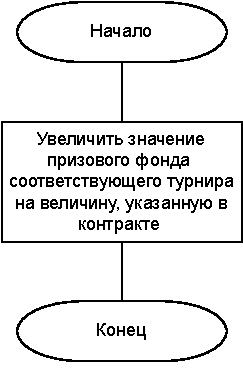
\includegraphics{inc/diag/new_sponsorship.pdf}
	\caption{Схема триггера обновления призового фонда турнира}
	\label{fig:new_sponsorship}	
\end{figure}

При добавлении записи о победе команды в рамках определенного турнира следует увеличивать величину общего заработка команды. Для этого используется триггер, схема которого приведена на рисунке \ref{fig:new_winner}.

\begin{figure}[h!btp]
	\centering
	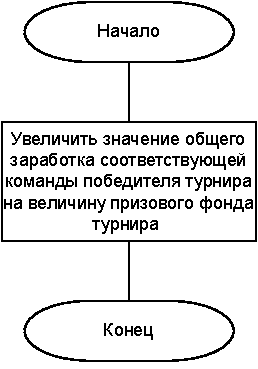
\includegraphics{inc/diag/new_winner.pdf}
	\caption{Схема триггера обновления общего заработка команды}
	\label{fig:new_winner}	
\end{figure}

\section{Выводы}

В данном разделе было выполнено проектирование базы данных, описаны таблицы, которые необходимо реализовать в рамках рассматриваемой задачи, а также разработаны схемы триггеров для базы данных.

